\documentclass[a4paper,12pt]{article}        
\usepackage[utf8]{inputenc}         
\usepackage[french]{babel}  
\usepackage[T1]{fontenc} %encodage de la police 
\usepackage[top=2.4cm,bottom=2cm,left=2.6cm,right=2.6cm]{geometry} %marges
\usepackage{graphicx} %affichage des images    
\usepackage{hyperref} %pour les liens
\usepackage{enumitem}
\usepackage[ruled, vlined, linesnumbered, french, onelanguage]{algorithm2e} %pour afficher un algorithme
\usepackage{listings} %pour afficher des lignes de code
\usepackage{xcolor} %ajoute de la couleur aux lignes de code
\usepackage{float} %pour placer correctement les images

\title{\textbf{Interpréteur de systèmes de Lindenmeyer}}
\author{LAVANDIER Augustin, FAUQUETTE Mael\\ KARKASHADZE Luka, MANDIN Paul\\ \\ L2 Informatique Groupe 4B}
\date{\today}
\pagenumbering{gobble}

\begin{document}

\maketitle
\begin{figure}[h]
\centering

\includegraphics[scale=1]{LOGO-UNICAEN_V-2.1-N.png}
\end{figure}

\newpage
\tableofcontents
\newpage
\pagenumbering{arabic}

\section{Introduction au projet}
\subsection{Description générale de la consigne du projet}

Ce projet avait pour but de nous faire développer un interpréteur de systèmes de Lindenmeyer, que nous appellerons LSystem pour le reste de ce rapport.
Tout d'abord, rappelons ce que sont les LSystem: ce sont des algorithmes permettant de représenter l'évolution de modèles végétaux selon des symboles et des règles.
\\\\
Effectivement, dans le monde des jeux vidéos ou du graphisme en général, il n'est pas rare de croiser des arbres, ou même des plantes. Ces LSystem permettent de les dessiner de façon plutôt simple. Chaque plante ou arbre est représenté par une suite de symbole, et chacun de ses symboles suit une règle qui lui ait propre. Et successivement à chaque évolution de cette plante, chaque symbole est analysé pour le faire suivre la règle qu'il connaît et donc faire pousser nos plantes ou nos arbres.

\subsection{Description de la problématique du projet}

Ce projet a pour but de réussir à nous faire comprendre comment fonctionne les LSystems et les utiliser avec des exemples concrets et faire en sorte de contrer les potentielles erreurs qui peuvent survenir. C'est pour cela que l'on a un modèle servant de base pour montrer que l'on maîtrise le concept de LSystem avec l'utilisation de règles, d'axium et d'occurrence. Et que l'on applique cette base sur une interface 2D et 3D de manière ergonomique et permettant de la personnalisation pour une utilisation concrète. Et pour finir, de nous entrainer à créer plusieurs tests permettant de vérifier l'intégrité de notre code.

\subsection{Présentation du plan du rapport}

Pour ne pas vous perdre lors de la lecture de ce rapport, voici les grands points qui y seront abordés et dans quel ordre:
\\\\
Tout d'abord nous continuerons cette courte introduction par la liste des objectifs qu'il fallait mettre en oeuvre pour compléter notre projet. 
Ensuite nous verrons les autres travaux en rapport avec ces L-Systèmes.
Nous verrons les fonctionnalités que nous avons implémentées dans notre interpréteur.
Nous verrons l'organisation de notre projet, c'est à dire comment nous nous sommes répartis les tâches tout au long de ce travail.
Suite à cela nous pourrons voir l'architecture de notre projet
Enfin nous arriverons sur les points techniques de notre interpréteur, nous verrons les librairies utilisées, nous décrirons les structures de données utilisées et les principaux algorithmes qui se doivent d'être expliqués pour une meilleure compréhension du fonctionnement.
Nous verrons des cas d'utilisation de notre projet et les tests que nous avons fournis.
Et enfin nous conclurons ce rapport.


\newpage
\section{Objectifs du projet}
\subsection{Présentation des objectifs à atteindre}

Il était assez important pour nous d'avoir dès le début de ce projet, une liste claire des différents éléments que nous devions mettre en place pour que ce projet soit totalement fonctionnel. C'est pourquoi nous avions la liste d'instructions à respecter qui est la suivante: 
\begin{itemize}[label=\textbullet, font=\small]
    \item Définir un langage pour construire un système de Lindenmeyer classique
    \item Implémenter un interpréteur pour une visualisation 2D
    \item Implémenter un interpréteur pour une visualisation 3D
    \item Étendre le langage et les interpréteurs pour des systèmes stochastiques et/ou contextuels
\end{itemize}
Nous avons fait au mieux pour respecter le maximum de ses consignes dans le temps qu'il nous a été donné.


\subsection{Autres travaux sur les L-Systèmes}

Pour nous aider lors de ce projet, nous avons utiliser toutes les ressources fournies lors des CM de conception logicielle. 

Et lorsque l'on parle de LSystem, nous sommes obliger de parler du livre "The Algorithmic Beauty
of Plants" écrit par Przemyslaw Prusinkiewicz et Aristid Lindenmayer. Ce livre nous a permit d'apprendre comment fonctionnait les LSystem, de la base à des choses plus compliquées comme la génération en 2D ou 3D. Dans ce livre, chaque question que nous nous posions y fusse déjà répondu à un endroit ou à un autre. Nous cherchions des exemples de mots et de règles a implémentés automatiquement ? Des exemples étaient fournis. Et de tous les types ! Que ce soit des mot stochastiques ou même des mots contextuels. L'ensemble des connaissances sur les LSystem y étaient stockées.



\section{Fonctionnalités implémentées}
\subsection{Explications des fonctionnalités}

Tout d'abord, pour lister les différentes fonctionnalités que possède notre projet, parlons tout d'abord des fonctionnalités de bases des LSystem.

Notre projet possède un modèle, un affichage 2D et un affichage 3D. Commençons par décrire les fonctionnalités de notre modèle. Notre modèle permet tout d'abord, de créer des mots fait de symboles, qui peut être lu, modifié selon des règles définies par l'utilisateur, être supprimé, ou même être enregistré. Notre mot modifiable peut suivre plusieurs règles à la fois, et surtout plusieurs règles pour une seule et même lettre. C'est à dire que dans les fonctionnalités implémentées, il y a bien entendu des règles normales, mais aussi des règles stochastiques, et enfin des règles contextuelles (dépendant de ce qu'il y a avant et après la lettre analysée). Pour continuer sur les fonctionnalités crées dans ce modèle, nous pouvons parler de notre WordBackUp, c'est un tableau enregistrant l'ensemble des mots que nous avons créés et modifiés et permet de gagner beaucoup de temps sur les modifications d'un même mot. 
\\\\\\
Maintenant pour ce qui est du mot en lui même, il est complètement modifiable par l'utilisateur, il peut créer ses propres règles, son propre axium (l'étape 0 du mot), sa propre WordBackUp. Ce mot, en plus d'être complètement personnalisable, il est modifiable à tout moment tout au long du code.
\\\\
C'est donc avec l'ensemble de ces mots que nous pouvons offrir la possibilité de dessiner nos premiers arbres. Comme dis précédemment notre projet a 2 fonctionnalités principales qui sont l'affichage 2D et l'affichage 3D.

L'interpréteur 2D se présente sous forme d'une interface principale où, sur le panel de droite sont dessinés les arbres et, le panel de gauche quelques options tel que des arbres prédéfinis, une entrée de texte pour définir la taille de l'arbre suivant, une barre de chargement, un bouton pour effacer tout les arbres sur le panel. Il y a un dernier bouton permettant d'afficher une interface tierce servant a créer nos propres arbres suivant des règles que nous pouvons définir et en créer plusieurs ainsi que les effacer. Pour afficher nos arbres, nous avons décidé d'utiliser le clic de la souris permettant de dessiner ainsi les arbres facilement avec les coordonnées du clic étant la racine de l'arbre.     

\subsection{Organisation du projet}

Au début du projet nous avons tous commencer a travailler sur les différentes classes de base d'un Lsystem, nous nous sommes lancer sur la création du modèle avec chacun une partie qui lui était désignée. Ceci n'était qu'une ébauche car beaucoup de nos créations du début furent supprimer par la suite. Une fois que le projet fut avancé et que Luka ait fini alphabet, il a commencé à travaillé sur la jFrame (les arbres 2D) suivit de Paul qui avait également finit sa partie. Mael quand a lui après avoir fini de travailler sur le modèle a commencé à faire des recherches sur la 3D et a trouvé la librairie LWJGL que nous utilisons actuellement. Ce travail sur la 3D lui a demandé beaucoup d'efforts et beaucoup de temps. Tous ces tests de librairies en compagnie d'Augustin leur ont permis de découvrir des dizaines de bibliothèques, mais LWJGL fut celle qui paraissait la plus agréable à manipuler. Augustin après avoir finalisé les base de notre projet et après avoir abandonner Mael dans la 3D, a rejoint Paul sur la 2D et avancé l'interface 2D du projet. A la fin de notre projet Luka et Mael travaillaient principalement sur la 3D, tandis que Paul et Augustin se penchaient plutôt sur les contrats du code, le modèle a peaufiner, et les tests unitaires à finir.
\\\\
Pour présenter rapidement comment sont triés nos dossiers, et nos class. Nous avons suivis la base du cours, c'est à dire que nous avions deux grands dossiers: ./branch et ./trunk. Branche était le dossier dans lequel nous faisions toutes les modifications au fur et à mesure, sans trop se soucier de si le code fonctionnait ou non. Quand à Trunk, se fut le dossier dans lequel nous mettions chaque version opérationnelle du code. Il fallait que le code s'exécute correctement avant de se décider à le mettre dans ./trunk. Ensuite, nous avions une partie ./src qui contenait le code, c'est à dire nos packages et nos class. Un dossier ./bin qui permettait de stocker les executables. Ensuite un dossier ./lib qui permettait de garder nos librairies. Le dossier ./doc qui permet de stocker la javadoc de notre projet. Et enfin un dossier ./ressources dans lequel se trouvait se rapport et quelques autres fichiers.


\newpage
\section{Architecture du projet}
\subsection{Diagramme des divers modules et classes}

 Voici le diagramme de l'ensemble de nos packages et nos class pour les comprendre plus clairement:

\begin{figure}[h]
\centering
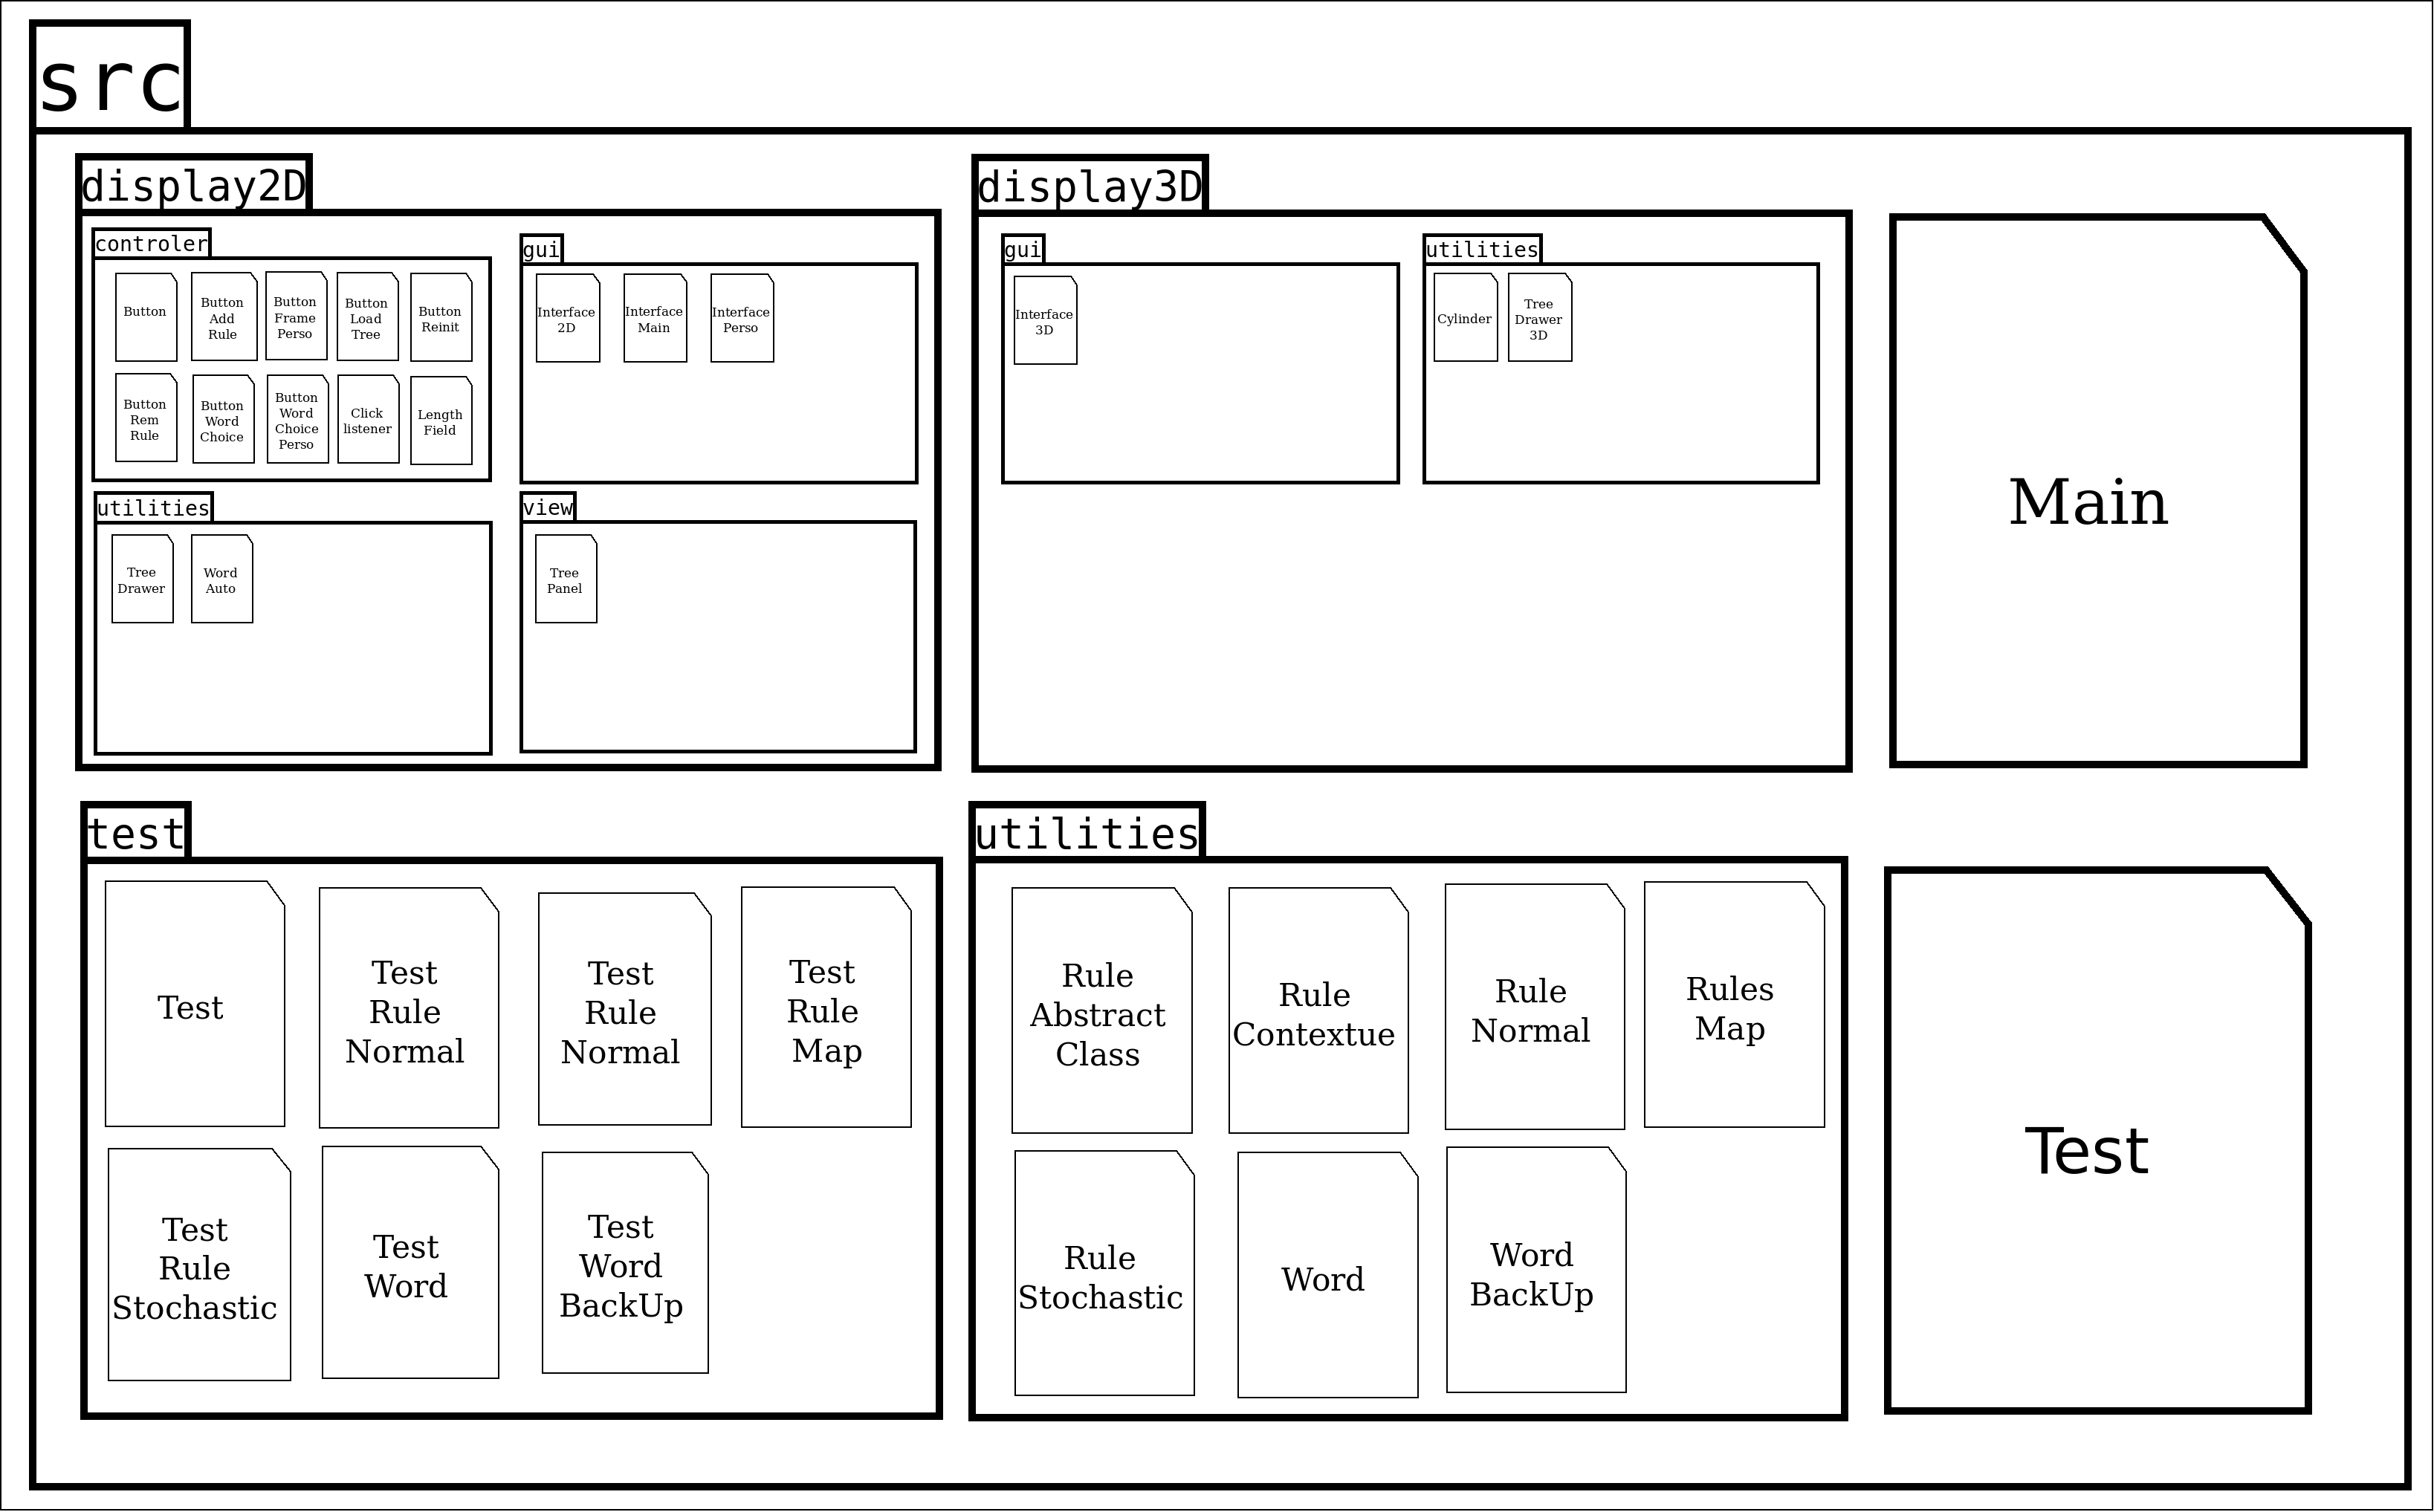
\includegraphics[scale=0.155]{Diagram_packages}
\end{figure}

Pour expliquer rapidement nos choix dans le rangement de nos class et de nos packages: pour débuter, nous avons séparer les class exécutables directement dans le packages src. Ensuite, nous avons le package de test permettant simplement de tester notre programme, et n'aurait rien eu à faire mélanger dans d'autres packages.
\\\\
Pour ce qui est du reste, nous nous sommes inspirés, dès que nous avons appris l'existence de cette méthode, de la MVC (modèle vue controller). C'est à dire que le package utilities est notre "modèle", il est utilisable sans avoir les vues et se charge en grande partie de faire tous les calculs lourds et techniques. 
\\\\
Enfin, nous avons les packages display2D et display3D, qui chacun d'entre eux est censer contenir des vues, permettant d'afficher nos arbres en 2D ou en 3D; des controllers, servant de boutons, ou de clickListener pour actionner notre modèle; des utilities, servant de sous modèles dans des cas précis pour notre affichage ;et enfin des gui, permettant de faire le lien entre le tout.

\newpage
\section{Éléments techniques}

\subsection{Description des diverses librairies utilisées}
La seule bibliothèque que nous utilisons est LWJGL qui est une bibliothèque de programmation graphique utilisée pour créer des images 3D interactives. Nous utilisons LWJGL car c'est une des bibliothèques qui nous fournissait le plus de possibilités pour coder. Car en effet, cette bibliothèques est directement en lien avec d'autres bibliothèques très connues comme OpenGL ou même Vulkan. 
\\\\
Nous utilisons donc LWJGL, ce qui nous permet de créer une fenêtre avec des objets 3D mouvants à l'intérieur. Elle nous permet d'afficher des cylindres qui représentent les troncs et les branches de nos arbres. 
\subsection{Description des diverses structures de données}

Dans notre projet nous utilisons différentes structures de données dont certaines de manière récurrente:

\begin{itemize}[label=\textbullet, font=\small]
    \item Pour commencer par le modèle, nous avons fait le choix de créer nos propres structures de données. Tout d'abord les différentes Rules, qui permettent de modifier un mot selon ce qui les définies. Il existe plusieurs types de Rules, mais ils héritent tous d'une même class abstraite: RuleAbstractClass. Chaque règle possède donc au moins une clef et une valeur qui en réalité, le "avant / après" modification de la lettre en question. Ensuite, nos Rules sont triées grâce à une autre structure de données, une RulesMap. Son nom est trompeur, car on pourrait penser que cette class hérite directement de la class HashMap, mais non. Simplement cette class ne possède qu'un seul attribut, qui est par contre une HashMap. Cette HashMap possède comme clefs, les valeurs des règles, et en valeurs, une liste de règles que doit suivre la lettre en question. Cette liste de règles est construite de la manière suivante: son premier élément est forcément soit une RuleNormal, soit une RuleStochastique. Le reste des éléments sont des RuleContextuel. Pour ce qui est du reste des structures de données que nous avons pu créer, nous avons bien entendu, les différents Word. Chacun de ces mots possède, un axium (sa phase 0), sa RulesMap, sa liste de lettres ignorées et sa WordBackUp. Enfin la WordBackUp, c'est un tableau à deux dimensions contenant des mots. Chaque liste de liste est une liste d'un même mot, ayant le même axium, les mêmes règles, mais à chaque fois à une occurrence supérieure. Cette WordBackUp nous permet d'enregistrer les mots déjà chargés et donc éviter un temps de chargement exponnentiel sous certaines conditions.
\\
    \item Au niveau de l'interface 2D il y a évidemment les JFrame ainsi que les Jpanel, mais on utilise aussi beaucoup des classes qui extends de JButton pour une utilisation plus simple et plus claire. Ainsi chaque bouton sur l'affichage 2D est en faite une classe étendue. Pour la JFrame de personnalisation on retrouve aussi des JTextField pour permettre de rentrer les valeurs que l'on souhaites pour nos arbres. Et pour les dessiner un ClickListener et un MouseListener sont utiliser pour récupérer les coordonnées du clic de la souris sur le panel pour servir de racine à l'arbre.
\\
    \item Les piles nous ont été très utile en 2D comme en 3D elle nous ont permis de sauvegarder les différentes coordonnées lors de la séparation de l'arbre en branches ainsi que la valeur de l'angle courant. Elles sont ensuite dépilée lorsque une branche se finit par exemple. 

\end{itemize}
\subsection{Description des principaux algorithmes}

Pour présenter désormais les principaux algorithmes, nous allons d'abord commencer par les algorithmes les plus importants du modèle:
\\
\begin{itemize}[label=\textbullet, font=\small]
    \item Pour commencer, une des idées que nous avons eu, c'est ce système de "Back Up des mots". Un système qui nous permet d'enregistrer tous les mots déjà chargés par la machine. La complexité de cet algorithme n'est pas à négliger, mais elle nous permet de gagner un temps immense sur la complexité exponentielle de chargement des mots. Mais comment fonctionne cet algorithme ?
    \\
    Tout d'abord, il faut savoir que nous avons deux grandes fonctions importantes dans cet algorithme, le reste est exécuté lors du chargement des mots. Ces deux méthodes très importantes sont: getLastWordLike() et addWordToList(). 
    getLastWordLike() est plutôt simple à comprendre, le but de cette fonction est de retrouver dans la back up, le mot déjà chargé et étant le plus proche de celui qu'on essaye de charger. C'est à dire que nous cherchons un mot qui a le même axium, les mêmes règles, et qui a un nombre d'occurence le plus de proche du nombre d'occurence final au chargement. Ce qui signifie que si nous avons déjà un mot ayant le même début (sous entendu le même axium) que celui cherché et ayant une occurence plus grande, nous n'avons pas besoin de charger le mot recherché. Et si l'occurence est plus petite, mais simplement de quelques occurences, cela nous fera forcément gagner du temps sur le chargement.
    \\\\
    Maintenant pour ce qui est de addWordToList(), pour comprendre cette méthode, il faut avoir en tête comment est construite la backUp (pour les trous de mémoire, il faut remonter au point précédent 5.2). Cette méthode ajoute donc au tableau wordList, le mot mit en argument s'il n'est pas déjà dedans. Pour se faire, nous parcourons l'ensemble des mots présents dans le tableau et regardons jusqu'à trouver un mot ayant le même début ou dans le cas contraire, on ajoute directement une nouvelle liste contenant ce nouveau mot. Mais si nous trouvons un mot ayant le même début, nous n'avons plus qu'à regarder si un nombre avec autant d'occurrences est déjà présent, auquel cas rien ne se passe, sinon, le mot est cloné pour éviter des problèmes de pointeurs et est ajouté au tableau wordList.
    \\
    \item Lorsque l'on nous demande quel est l'algorithme le plus important que nous avons pu coder dans cet interpréteur de LSystems, comment ne pas penser directement à l'algorithme permettant de faire évoluer les mots ? Pour l'expliquer simplement, cette méthode permettant cela est la méthode readAndApplyRulesToWord() de la class Word. Cette méthode subie une surcharge, mais elle peut ne pas prendre d'arguments et va donc appliquer une occurrence au mot choisi, sinon, on peut choisir le nombre d'occurrences qui seront appliquées, et on peut aussi choisir d'afficher la progression du chargement dans une JProgressBar, cela est utile pour l'affichage des arbres en 2D. 
    \\\\
    Pour commencer à décrire l'algorithme, tout d'abord nous regardons si le mot n'est pas déjà connu de la BackUp, ou si elle ne connaît pas un mot similaire avec un peu moins d'occurrences de façon à limiter les calculs très gourmands qui arrivent. Une fois que nous avons trouvé quelque chose ou rien du tout, nous rentrons dans une boucle (sauf dans le cas ou le mot est déjà trouvé). Cette boucle for nous permet de parcourir le nombre de fois souhaité le mot pour le faire évoluer du nombre d'occurrences voulues. Une fois que nous commençons à parcourir le mot, nous devons définir un mot temporaire vide, qui prendra comme valeur le nouveau mot petit à petit. Nous récupérons la lettre à traiter, la lettre précédente et la lettre suivante pour gérer les règles contextuelles. Les lettre précédente et lettre suivante sont analysées de façon à ce que des lettres présentes dans la liste "ignored" ne soient pas prises en comptes. Une fois que toutes les variables sont stockées, on vérifie si il existe une règle contextuelle dans la situation présente, si c'est la cas, nous appliquons la règle en ajoutant sa valeur au mot temporaire, si ce n'est pas le cas, nous ajoutons la valeur de la règle normale de la lettre au mot temporaire. Une fois que tout le mot est analysé et parcourus de cette manière, nous lui ajoutons une occurrence, et recommençons tant que la boucle for n'est pas finit. 
\\\\\\
    Une fois cela effectué, nous finissons ce tour de boucle par l'ajout dans la backup du mot que nous venons de créer et nous relançons la boucle.
    \\
\end{itemize}

Dans la liste des principaux algorithmes que nous utilisons, nous pouvons retrouver encore:
Le principe des threads qui permettent d'effectuer plusieurs taches en même temps:\\
\begin{itemize}[label=\textbullet, font=\small]
    \item l'InterfaceMain qui n'est pas un thread mais qui gère l'affichage des arbres sur le PanelTree
    \item un 1er thread qui se lance lorsque l'on clique sur le bouton d'affichage de la frame auxiliaire de personnalisation. permettant ainsi d'afficher, d'utiliser et de connecter les 2 frames en simultanée
    \item un 2eme thread qui se lance lorsque l'on clique sur le bouton de chargement d'un arbre. Étant donné que c'est un thread, pendant qu'un arbre charge il est totalement possible de continuer de dessiner sur l'InterfaceMain.\\
\end{itemize}



Pour dessiner un arbre il nous faut un mot complet crée grâce à l'algorithme vu si dessus(integrer readAndApply). Ce mot est composé de motif ayant différentes règles pour le dessin:
\begin{itemize}[label=\textbullet, font=\small]
    \item "F" : permet de dessiner un trait du point de départ vers un point B
    \item "+" : permet de changer l'angle vers la gauche suivant l'angle de l'arbre
    \item "-" : permet de changer l'angle vers la droite suivant l'angle de l'arbre
    \item "[" : permet de sauvegarder la position du point actuel
    \item "]" : permet de de revenir à la position du point sauvegardé\\
\end{itemize}
Ainsi pour dessiner un arbres il suffit de parcourir le mot motif par motif et suivre la règle de chaque motif.

Pour la création des arbres en 3D , nous avons tout d'abord développé des cylindre 3D qui nous serviront de branches élément constitutif des arbres en 3D. Les cylindres ont un fonctionnement plutôt simple le cylindre se crée à une coordonnée d'abscisse X, d'ordonnée  Y et de profondeur Z. Ensuite en prennent en compte ces coordonnés des quadrilatères sont créer à 360° ce qui affiche un cylindre, sa création ce fais dans le fichier Cylindre.java.  
\\\\
Pour dessiner un arbre en 3D, il nous faut un mot complet crée grâce à l'algorithme vu si dessus. (integrer readAndApply). Ce mot est composé de motif ayant différentes règles pour le dessin:\\
\begin{itemize}[label=\textbullet, font=\small]
    \item "F" : permet de créer un cylindre avec comme point de départ son milieu
    \item "+" : permet de changer l'angle vers la gauche sur l'axe Y suivant l'angle de l'arbre
    \item "-" : permet de changer l'angle vers la droite sur l'axe Y suivant l'angle de l'arbre
    \item "$\backslash$" :permet de changer l'angle vers la gauche sur l'axe Z suivant l'angle de l'arbre
    \item "/": permet de changer l'angle vers la droite sur l'axe Z suivant l'angle de l'arbre
    \item "\&": permet de changer l'angle vers la gauche sur l'axe X suivant l'angle de l'arbre
    \item "$\wedge$": permet de changer l'angle vers la droite sur l'axe X suivant l'angle de l'arbre
    \item "|": permet de changer l'angle vers la droite sur l'axe Y suivant un angle de 180°
    \item "[" : permet de sauvegarder la position du point actuel
    \item "]" : permet de de revenir à la position du point sauvegardé\\
\end{itemize}
Chaque éléments du mot doit modifier les cylindres, en changent l'orientation ou les coordonnées ou en affichant 
 ces dernier lorsque cela est nécessaire. En cela la classe TreeDrawer3D.java permet la lecture du mot et l'application des instructions aux cylindres. La rotation est effectué grâce à glRotatef qui prend en argument les angles angleX, angleY et angleZ qui permet une rotation sur l'axe associé au nom de ces variable et le placement quand à lui est gérer par glTranslatef qui permet de positionne les cylindres aux coordonnées mis à jours après lecture de chaque éléments.
 \\\\Pour ce qui est de la sauvegarde de la position elle est faite grâce a un Stack dans TreeDrawer3D.java ainsi qu'avec la classe Pose.java qui renvoie x, y, z, angleX, angleY et angleZ. 
Ainsi pour dessiner un arbres il suffit de parcourir le mot motif par motif et suivre la règle de chaque motif

\newpage
\section{Expérimentation et usages}

\subsection{Cas d'utilisation}

Il existe trois manière d'utiliser notre interpréteur de LSystem, tous trois accessible après avoir ouvert un terminal dans le dossier trunk, et entrée cette commande : ant run
\begin{figure}[h]
\centering
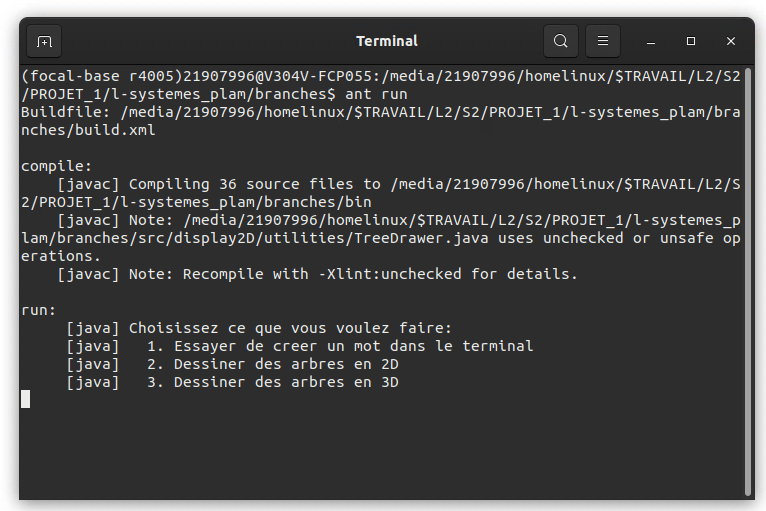
\includegraphics[scale=0.6]{Gameplay/ant_run.png}
\end{figure}

Comme indiqué ci-dessus il vous faut rentré 1, 2 ou 3 qui lance respectivement en shell, en 2D (jFrame) ou en 3D (lwjgl).
\\
Voici une session en shell (1) :

\begin{figure}[h]
\centering
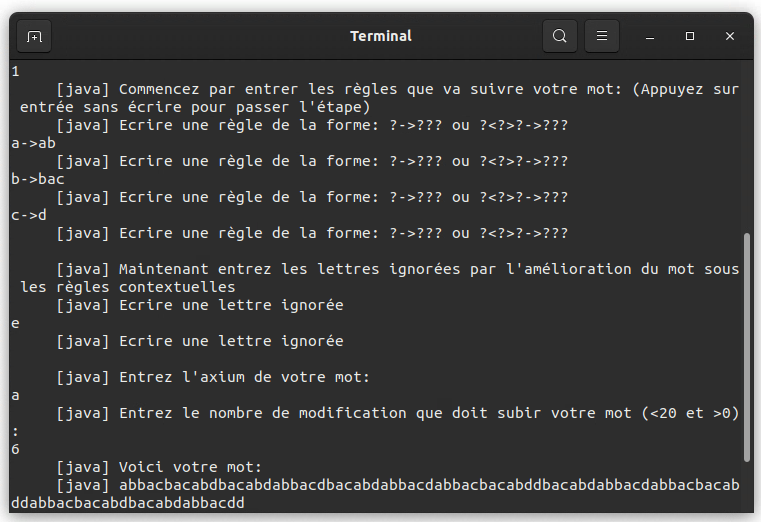
\includegraphics[scale=0.6]{Gameplay/1D_tree.png}
\end{figure}

\newpage
Il est également possible de lancer une session en jFrame (2): 
\begin{figure}[h]
\centering
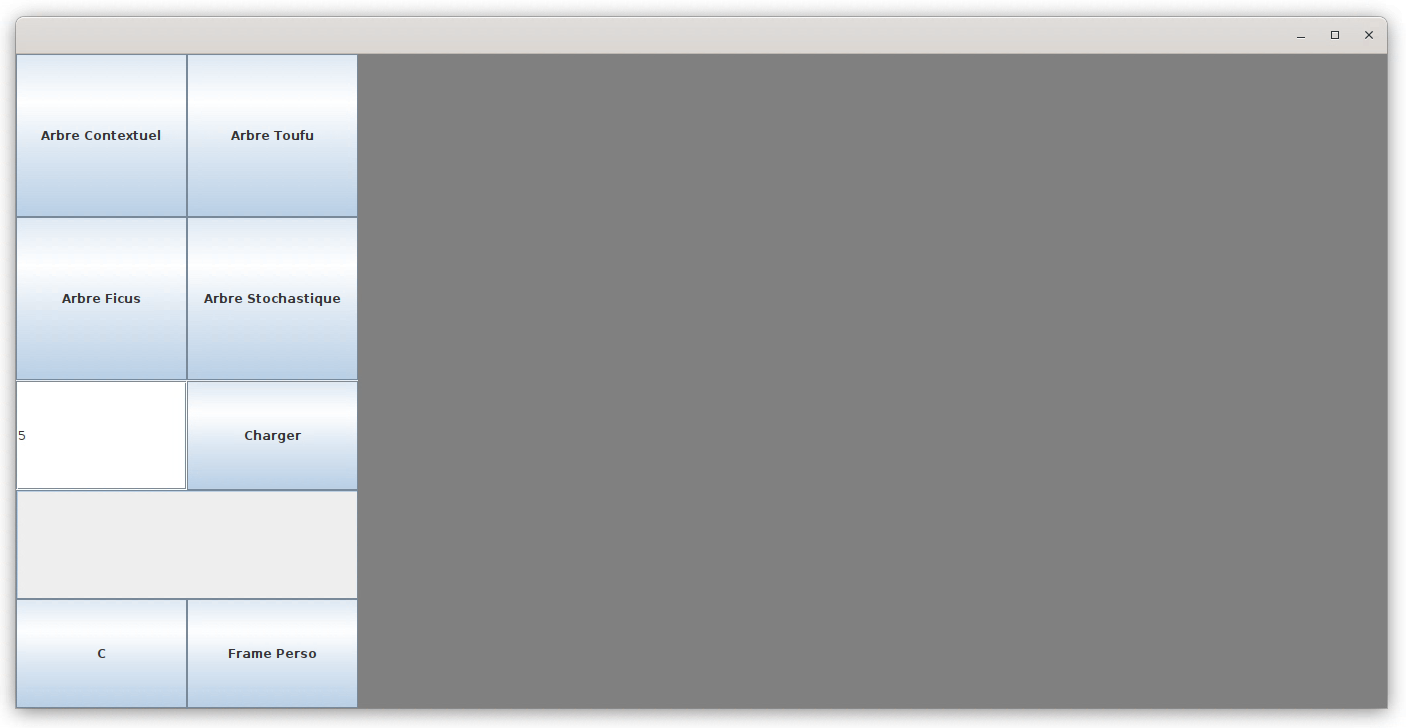
\includegraphics[scale=0.48]{Gameplay/2D_start.png}
\end{figure}

Dans cette session, il est possible de créer plusieurs arbre dans la partie grise. Pour créer un arbre il faut cliquer sur le bouton correspondant à l'arbre, puis le charger grâce au bouton charger en ayant au préalable définit le nombre d'occurrences souhaité pour ce dernier. 
\\\\
Il est ainsi possible d'avoir plusieurs arbre diffèrent à l'écran. Nous avons deux arbre "spéciaux" un arbre contextuel dont les élément dépendes les un des autres et un arbre stochastique qui dépendes des probabilités aléatoires :

\begin{figure}[h]
\centering
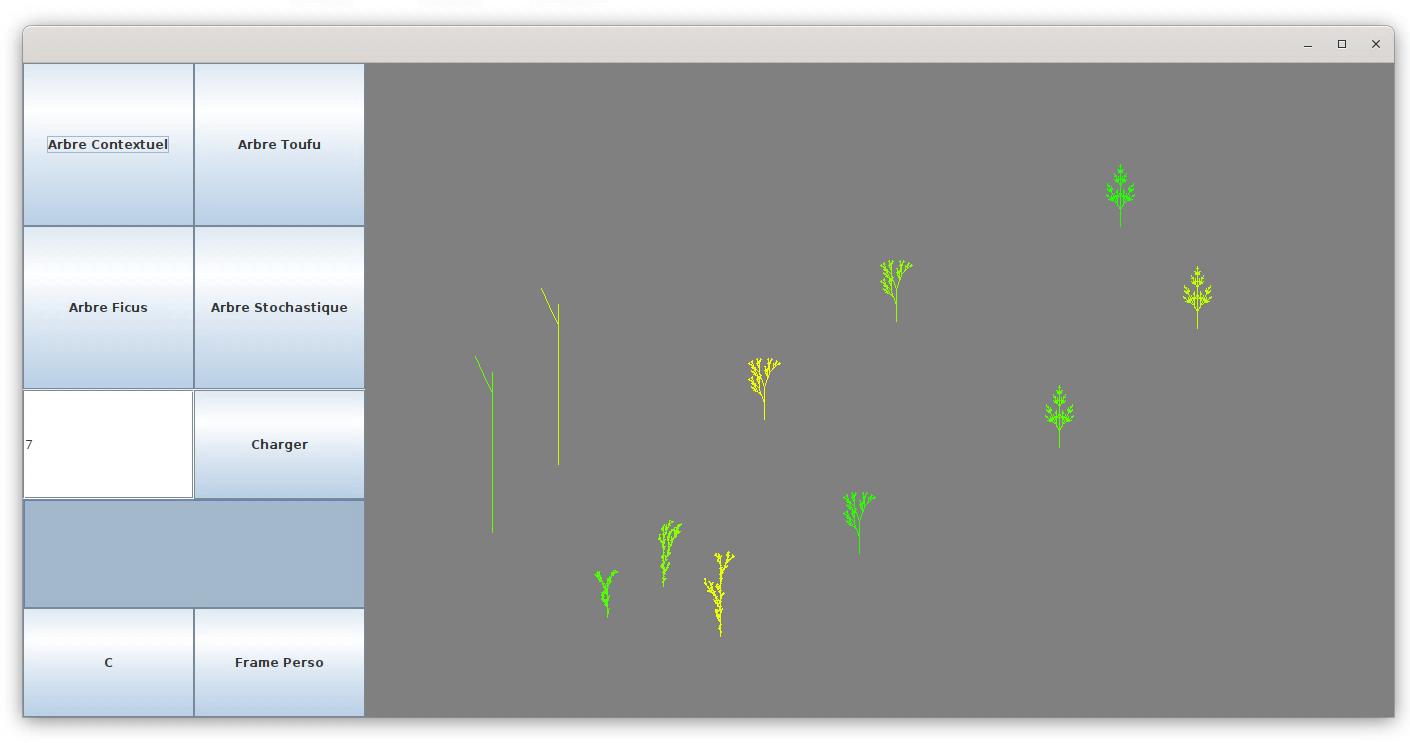
\includegraphics[scale=0.48]{Gameplay/2D_tree.png}
\end{figure}
il existe la possibilité de nettoyer le panneau d'affichage grâce au bouton "C" (Clear).
\\\\
De plus comme pour la session en shell, il est également possible de créer ses propres arbres grâce au bouton "Frame Perso" :
\begin{figure}[h]
\centering
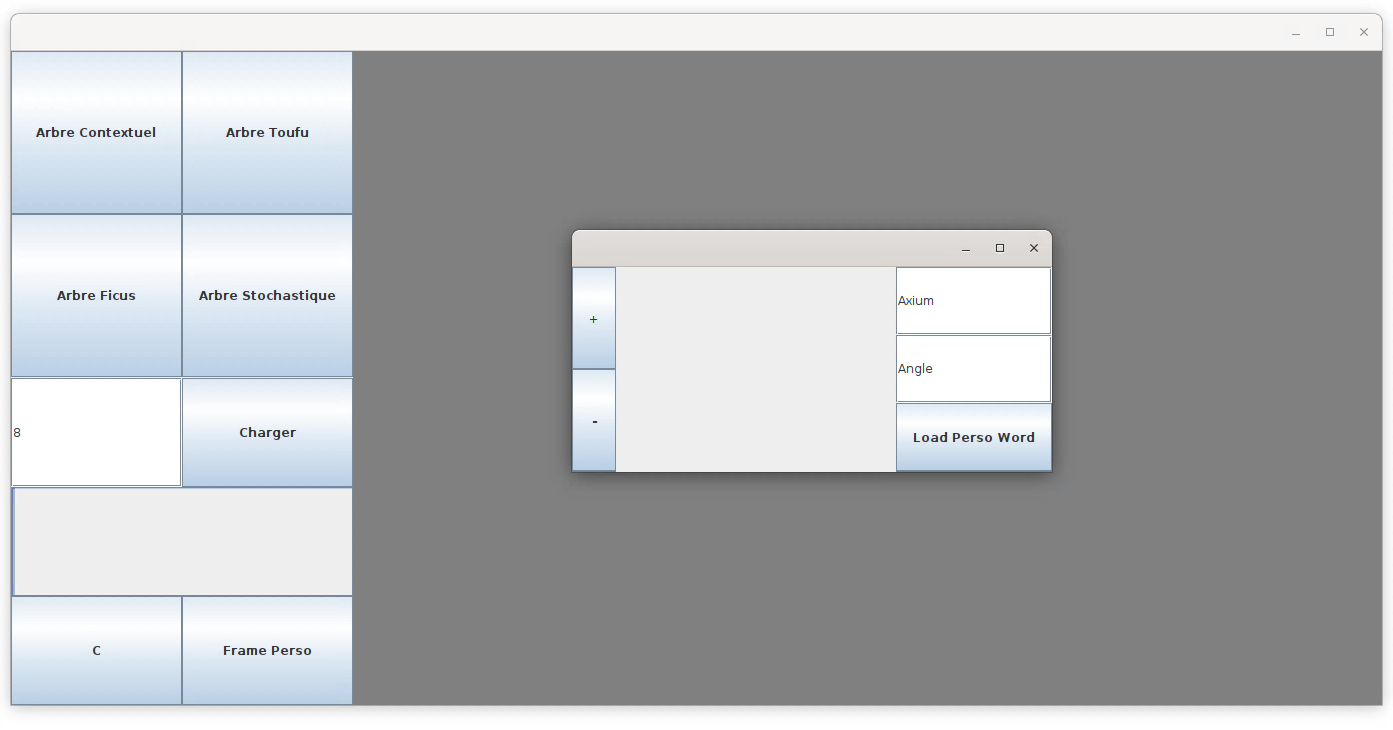
\includegraphics[scale=0.48]{Gameplay/2D_tree_perso.png}
\end{figure}
la partie 3D est de loin la partie qui nous a posé le plus de problèmes, cependant même si toutes les règle n'ont pas pu être correctement implémente le rendu des arbres 3D reste tout de même agréable :

\begin{figure}[h]
\centering
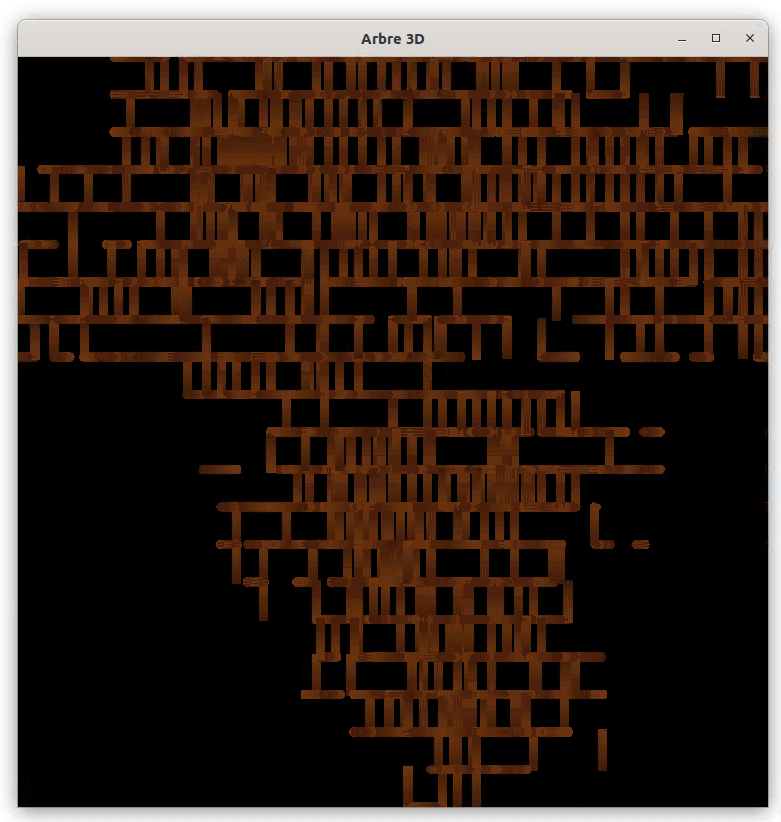
\includegraphics[scale=0.42]{Gameplay/3D_tree.png}
\end{figure}

\newpage
Pour vérifier si nos fonction était fonctionnelles des test unitaire ont été fait leur resultat est accessible par l'ouverture d'un terminal dans le dossier trunk, en entrant la commande : ant test

\begin{figure}[h]
\centering
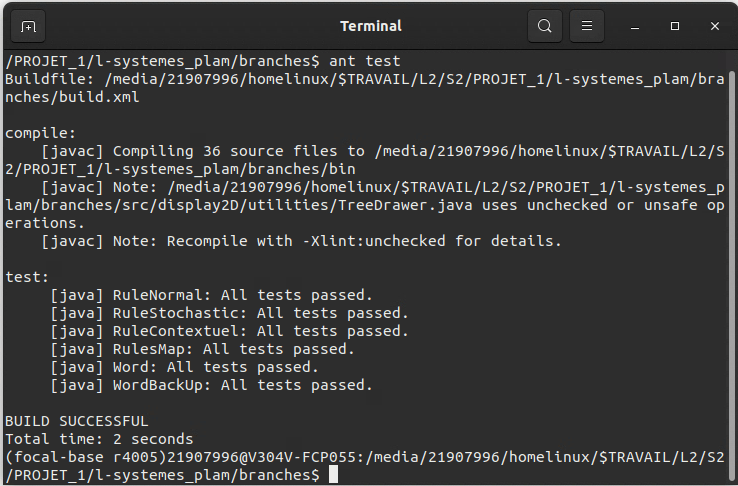
\includegraphics[scale=0.6]{Gameplay/ant_test.png}
\end{figure}
\subsection{Jeux de tests}

Maintenant pour ce qui est des jeux de tests. Nous utilisons la méthode la plus simple possible. C'est à dire que nous testons toutes les classes du modèle de notre interpréteur. Et pour les tester, nous faisons simplement quelques tests unitaires sur chaque méthode de chaque class.
\\
Prenons par exemple la class TestRuleNomral.java:
\\
\begin{lstlisting}[language=Java, numbers=left, basicstyle=\ttfamily\footnotesize, keywordstyle=\color{blue}\ttfamily, stringstyle=\color{red}\ttfamily, commentstyle=\color{green}\ttfamily,
numberstyle=\tiny, frame=single, linewidth=12cm]
public static void launchTest(){

        try{
            //Initialisation de la class
            RuleNormal ruleTest1 = new RuleNormal(...);
            RuleNormal ruleTest2 = new RuleNormal(...);
            RuleNormal ruleTest3 = new RuleNormal(...);

            //Tests des fonctions ...

            assert ruleTest1.getRule() == ...:"Error";
            
             System.out.println("RuleNormal: All tests
passed.");

        } catch(Exception e){
            System.out.println(e);
        }

    }
\end{lstlisting}
\newpage
Dans cet exemple, nous créons plusieurs règles de tests ayant chacune des propriétés différentes de façon à tester l'ensemble des possibilités avec nos méthodes. Ce bloc de test de méthodes se trouve dans un try, ce qui permet de, si une erreur survient, le code se stoppera de lui même et les restes des tests ne s'exécutera pas. 
De plus, nous avons fait le choix de tester notre code via des asserts, car ils sont plus simples à gérer et à comprendre que des erreurs classiques. Ils permettent de ne pas ralentir le code si l'on ne veut pas les prendre en compte. Mais cela oblige à rajouter un paramètre lors de l'exécution de notre code (ici le problème ne se pose pas, puisqu'il suffit simplement de lancer la commande "ant test" depuis le dossier ./trunk pour compiler et exécuter les tests).
\\\\
Ces tests sont donc très simplistes, mais ils font tout de même l'affaire et permettent tout de même d'avoir une bonne idée de si notre code fonctionne toujours ou non.


\section{Conclusion}

\subsection{Récapitulatif des fonctionnalités principales}

Pour récapituler assez rapidement les fonctionnalités que nous avons réussi à mettre en place.
\\\\
Tout d'abord, nous avons un modèle complet. C'est à dire que nous pouvons créer des mots, les modifier, les supprimer. Créer nos propres règles. Sauvegarder nos mots pour gagner en complexité sur le long terme. Nous avons de plus, des tests unitaires assez simples et fonctionnels permettant de vérifier que l'ensemble de notre code fonctionne. 
\\\\ 
Ensuite, nous avons réussi à adapter notre modèle à l'affichage des arbres en 2D. Encore une fois, l'interface est adaptée à la personnalisation pour l'utilisateur. Il peut choisir des mots prêts-faits, comme il peut faire ses propres arbres avec ses règles et ses valeurs. 
\\\\
Enfin, nous avons essayer d'adapter ce système de mot à une interface en 3D. Cela a été très difficile à mettre en oeuvre et a pris beaucoup de temps à être mis en place. Nous ne sommes pas arrivés à un affichage d'arbres fonctionnels car nous avons encore des problèmes pour ce qui est des angles et de certaines coordonnées, mais certains arbres très simples peuvent fonctionner.

\subsection{Propositions d'améliorations}

Maintenant, nous allons voir l'ensemble des points d'améliorations que nous aurions aimé mettre en place pour améliorer ce projet.
\\\\
Il est vrai que dans notre situation, l'amélioration de la 3D qui n'a pas pu être finie par manque de temps, fait que c'est un des points d'amélioration que nous travaillerions en priorité. Effectivement, après en avoir discuté plusieurs fois avec le reste du groupe, c'est le point le plus frustrant dans ce projet, malgré tous les efforts mis dans cette partie de notre code, nous n'avons pas réussi à en venir à bout.
\\\\
Ensuite, nous aurions pu améliorer la personnalisation de la 3D par l'utilisateur. Faire tout comme nous l'avions fait pour les arbres en 2D, mais en 3D, ce qui permettrait une plus grande maniabilité pour l'utilisateur.
\\\\
Enfin, nous aurions pu faire des mesures sur la vitesse d'exécution du code, cela nous aurait peut être permis d'améliorer l'efficacité de certains de nos algorithmes triviaux ou même de nos structures de données.
\\\\\\
Merci d'avoir lu ce rapport, en espérant que notre projet vous ait plus et intéressé. 

\end{document}